\paragraph{Experimente:}
\begin{itemize}
  \item gleichnamige Pole stoßen sich ab
  \item ungleichnamige Pole ziehen sich an\\
  \item Kraftwirkung $\propto\frac{1}{r^2}$ (1750; Coulomb)
  \item ähnliche Abstandsabhängigkeit für elektrische und für magnetische Kräfte
  \item zunächst kein Zusammenhang zwischen beiden Kräften erkennbar
  \item Experiment: Magnetische Pole treten nur paarweise auf. \\ ($\implies$ keine "magnetische Ladung")
\end{itemize}

\paragraph{Feldlinien sichtbarmachen durch Eisenfeilspitzen:}\leavevmode \\

\boxed{Magnetische Feldlinien sind stets geschlossen; es gibt keine isolierbaren Quellen oder Senken des magnetischen Felds.}

\paragraph{Erinnerung: Satz von Gauß:}\leavevmode \\
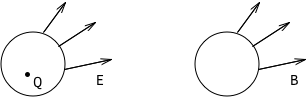
\includegraphics{skizzen/16/16_0B01}

$\vec{E}:$ elektrische Feldstärke:\\
Gesamtfluss: $\phi_{el}=\oint_A \vec{E}\cdot d\vec{A}=\frac{Q}{\epsilon_0}$\\

\subparagraph{Magnetische Felder:}\leavevmode \\

Gesamtfluss: $\boxed{ \phi_{mag}=\oint_A \underbrace{\vec{B}\cdot d\vec{A}}_{\text{magnetischer Fluss}}=0 \\ \vec{B}: \text{magnetische Flussdichte}}$
  
  \subsection{ Kräfte auf bewegte Ladungen }  
    \subsubsection{ Lorentzkraft $\vec{F}_L$ }
    $\vec{F}_L = q\cdot\vec{v}\times\vec{B}\\ (\vec{F}_L \perp \vec{v}; \vec{F}\perp \vec{B} ) $\\
    
    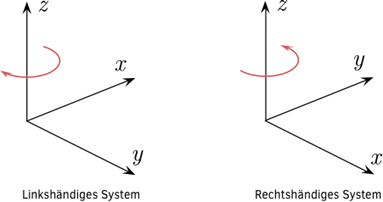
\includegraphics{skizzen/16/16_1B01}\\
    
    UVW-Regel: Ursache $\rightarrow$ Vermittler $\rightarrow$ Wirkung\\
    Vorsicht!: Elektrische Ladung ist negativ!\\
    
    $[\vert\vec{B}\vert]=\frac{N}{As\cdot\frac{m}{s}}=\frac{Vs}{m^2}=1T (Tesla)$
    
    Kreisbahn: $\vec{F}_L\perp \vec{v}$
    
    $\implies \vec{F}_L$ beeinfluss die Richtung von $\vec{v}$, aber nicht den Betrag!\\
    $\implies \vec{F}_L$ leistet keine Arbeit
    
      \paragraph{Konventionen:}\leavevmode \\
      
      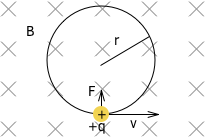
\includegraphics{skizzen/16/16_1B02}\\
      
      $\otimes \vec{B}$ zeigt in die Papierebene hinein\\
      
      $\odot \vec{B}$ zeigt aus der Papierebene heraus\\
      
      
  \subsubsection{Bewegungsgleichung:}\leavevmode \\
  
  $m\ddot{\vec{r}} = \dot{\vec{r}}=\vec{F}_L=q\cdot\vec{v}\times\vec{B} $\\
  
  $\frac{d\vec{v}}{dt}=\dot{\vec{v}}=\frac{\dot{\vec{p}}}{m}=\frac{q}{m}\cdot\vec{v}\times\vec{B}$\\
  
  $d\vec{v}\perp \vec{v}; d\vec{v}\perp\vec{B}$\\
  
  $\implies$  Kreisbahn: $\vec{F}_L$ ist Zentripetalkraft\\
  
  $\implies q\cdot v\cdot B=m\cdot\frac{v^2}{r}; v=\omega\cdot r$\\
  
  $\boxed{\omega=\frac{q}{m}\cdot B}$\\
  
  $\boxed{\nu=\frac{1}{2\pi}\cdot\frac{q}{m}\cdot B}$\\
  
  $\omega$ Zyklotronfrequenz (1930, Lawrence)\\
  
  $\implies$ unabhängig von Impuls und Energie; nur von $\frac{q}{m}$ und $\vec{B}$ bestimmt!\\
  
  \paragraph{Radius:}\leavevmode \\
  
  $r=\frac{m\cdot v}{q\cdot B}=\frac{p}{q\cdot B}= \frac{\sqrt{2mqV}}{q\cdot B}$\\
  
  $E_{kin}=\frac{p^2}{2m}=\frac{1}{2}m\cdot v^2=q\cdot V$\\
  
  \subparagraph{Experiment:}\leavevmode \\
  
  $r_1: V_1=200V\implies 2SKT$\\
  
  $r_: V_1=300V\implies 2,5SKT$\\
  
  $\frac{r_1}{r_2}\overset{!}{=} \sqrt{\frac{V_1}{V_2}}$\\
  
  $\frac{4}{5}\overset{!}{=}\sqrt{\frac{2}{3}}$\\
  
  $\frac{16}{25}\overset{!}{=}\frac{2}{3}$ \checkmark im Rahmen der Messungenaugikeit!
  
  \subsubsection{Zyklonen:}\leavevmode \\
  Ziel: H- oder D-Kerne auf hohe Geschwindigkeit zubeschleunigen.\\
  
  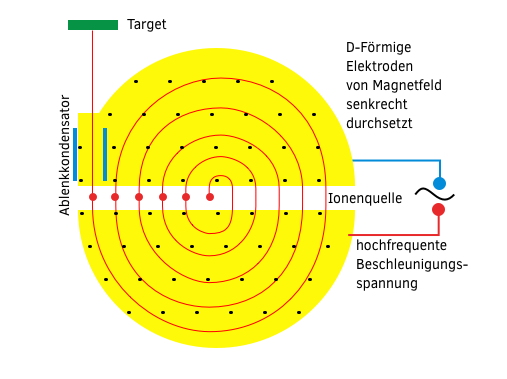
\includegraphics{skizzen/16/16_1B03}\\
  
  \paragraph{Beispiele:}\leavevmode \\
  (i) Protonenbeschleunigung: $r=0,5m; B=1,5T$\\
  Zyklonenfrequenz: $\nu\frac{e\cdot B}{2\pi m_0}=23MHz$\\
  
  $E_{kin}=\frac{1}{2}\frac{q^2 B^2}{m_0}\cdot v^2=4,3\cdot 10^{-1}J$\\
  
  Angabe in Elektronenvolt $\begin{align}
  	[eV]:1eV&= 1,602\cdot 10^{-19}As \cdot 1V\\
  	&=1,602\cdot 10^{-19}J
  \end{align}$\\
  
  $\implies \underline{26,9MeV}$\\
  
  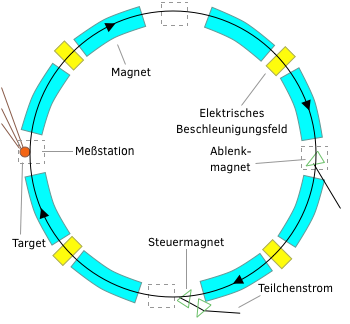
\includegraphics{skizzen/16/16_1B04}\\
  
  (ii) Massenspektrometer: Trennung von Isotopenmasser und Messung natürlicher Isotopenverhältnis:
  
  Beschleunigung (auf höhere E_{kin}) ist nur im elektrischen Feld möglich! ($\implies$ Design von Beschleunigung!)
  
  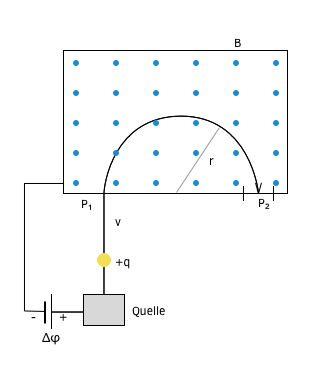
\includegraphics{skizzen/16/16_1B05}\\
  
  (Ashton 1919; $\frac{\Delta m}{m}=10^{-4})$\\
  
  Beispiel: Mg-Isotop: $\sideset{^24}Mg:78,7\%\\ \sideset{^25}Mg: 10,1\% \\ \sideset{^26} Mg: 11,2\% \\$
  Massenverhältnis: 24:25:26\\
  
  $\frac{q}{m}$ von Ionen bei bekannter Ladung: U
  $\begin{itemize}
  	\item \text{Beschleunigung:} q\cdot\Delta\varphi\implies E_{kin}=q\cdot U= \frac{1}{2}mv^2\\
  	\item \text{Kreisbahn:} r=\frac{m\cdot v}{q\cdot B}
  \end{itemize}$\\
  
  $\implies q\cdot U= \frac{1}{2}v^2\cdot B^2\cdot q^2\cdot \frac{1}{m}$
  
  $\boxed{\frac{m}{q}=\frac{B^2\cdot v^2}{2U}}$
  
  (iii) Geschwindigkeits…: Gekreuzte elektrische und magnetische Felder (Wien-Filter)\\
  
  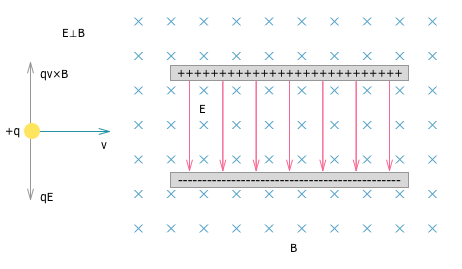
\includegraphics{skizzen/16/16_1B06}\\
  
  Kompensation der Felder ("Kräftegleichgewicht") für:\\
  $q\cdot E=q\cdot v\cdot B\\ \underline{v=\frac{E}{B}}$\\
  Ionen mit $v=\frac{E}{B}$ passieren die Anordnung ohne Ablenkung! ($\rightarrow$ Lochblende)\\
  Anwendungsbeispiel: SIMS\\
  
  \subsubsection{Kräfte auf stromdurchflossene Leiter}\leavevmode \\
  
        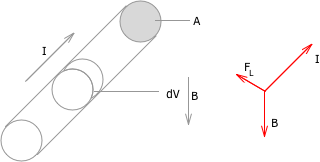
\includegraphics{skizzen/16/16_1B07}\\
        
        Kraft auf eine Ladung:\\
        $\vec{F}_L=q\cdot \vec{v}\times\vec{B}$\\
        
        Kraft auf N Ladungen in dV:\\
        $\begin{align}
        	d\vec{F}&= \underbrace{dV\cdot n}_{N}\cdot \vec{v}\times\vec{B}\\
        	&dV\cdot\vec{j}\times\vec{B}\\
        	\vec{F}_L&=\int_V(\vec{j}\times\vec{B})dV
        \end{align}$\\
        
        Geradliniger Leiter: Länge L\\
        
        $\vec{F}_L=\int_0^L(\vec{j}\times\vec{B}\underbrace{A\cdot dl}_{=dV}=\int_0^L(\vec{I}\times\vec{B})dl=\underline{(L\cdot(\vec{I}\times\vec{B})}$\\
        
        \paragraph{Leitersch…}\leavevmode \\
        Problem: Ladungsträgertyp nicht identifizierbar!\\
        $\implies$ Edmin Hall (1879): Hall-Effekt - Typ und Konzentration der Ladungsträger messbar!\\
        
        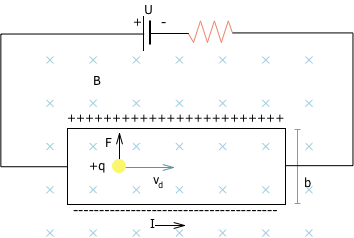
\includegraphics{skizzen/16/16_1B08}\\
        
        Annahme: positive Ladungsträger; Bewegung mit $\underline{\vert \vec{v}\vert=\vec{v}_D}$\\
        Gleichgewicht bei: $q\cdot \vec{v}_0\times \vec{B}+q\cdot\vec{E}_H=0\\ \vec{E}_H=-\vec{v}_0\times\vec{B}$\\
        
        Zugehörige Potentialdifferenz: U_H(Hall-Spannung):
        $\implies$ Polarität erlaubt Bestimmung des Ladungsträger-Types\\
        $\implies$ Dadurch konnte gezeigt werden, dass Ladungstransport in Metallen durch Elektronen erfolgt!\\
        
        $\vert \vec{E}_H\vert=\frac{U_H}{b}=\v_D\cdot B=\frac{n\cdot q\cdot v_D}{n\cdot q}\cdot B=\frac{j\cdot B}{n\cdot B}$\\
        
        Streifen der Dicke d: $j=\frac{I}{b\cdot d}$\\
        
        $U_H=\frac{I\cdot B}{n\cdot q\cdot d}=K_H\cdot\frac{I\cdot B}{d}$\\
        
        K_H:Hallkonstante (Materialspezifisch):\\
        $\boxed{K_H=\frac{1}{n\cdot q}=\frac{\mu}{\nu}}$\\
        
        $\implies$ Bei Kenntnis von $\nu$ ist $\mu$ zu bestimmen!
        
        \subparagraph{Cu-Streifen:}\leavevmode \\
        
        $I=4A; B=0,28T; d=2,0\mu m; U_H=50\mu V\\
        n_e=\frac{I\cdot B}{U_H\cdot q\cdot d}=\frac{4\cdot 0,28 A\frac{Vs}{m^2}}{50\cdot 10^{-4}V\cdot 1,6\cdot 10^{-19}As\cdot 2\cdot 10^{-6}m}\\
        =\frac{1}{1,6}10^{29}m^{-3}\\
        =\underline{…}$\\
        
        
        
        
        
        
        
        
        
        
        
        
        
        
        
\newpage  